\subsubsection{Latency \& Throughput}

Charts on Figures \ref{fig:sequential_app_latency}, \ref{fig:parallel_app_latency}, \ref{fig:sequential_app_throughput} and \ref{fig:parallel_app_throughput} represent the \gls{p90} of Latency and Throughput of all 10000 requests made by the sequential and parallel clients during the experiments.

\subsubsection*{High Parallel Client Latency}

The chart on Figures \ref{fig:sequential_app_latency} and \ref{fig:parallel_app_latency} shows latency has a similar behavior on both sequential and parallel clients, but their scale differ. Parallel clients show a hundredfold difference, as was also previously observed during transport-layer protocols experiments. This is a reflection of running 100 goroutines concurrently, requests takes longer to finish since each goroutine's request needs to wait for the other 99 requests to be processed by the host before it can be processed itself.

\subsubsection*{HTTP/1 performed better than HTTP/2}

During sequential experiments, HTTP/1 had a better latency and throughput than HTTP/2. Neither HTTP/1 pipelining nor HTTP/2 multiplexing had a big role during these experiments since they only improves parallel requests. Nonetheless, during parallel experiments, HTTP/1 still performed better than HTTP/2.

HTTP/1 pipelining allows clients to perform multiple requests in parallel \cite{rfc2616}, improving the overall time required to finish more than one request. However, responses must arrive in the same order as requests were made, therefore the first request must receive its response before the second does. This limits performance since a slow response can delay all other requests. HTTP/2 multiplexing solves this by allowing responses to arrive in any order (Figure \ref{fig:comparison_of_http_versions}).

\begin{figure}[h!]
    \centering
    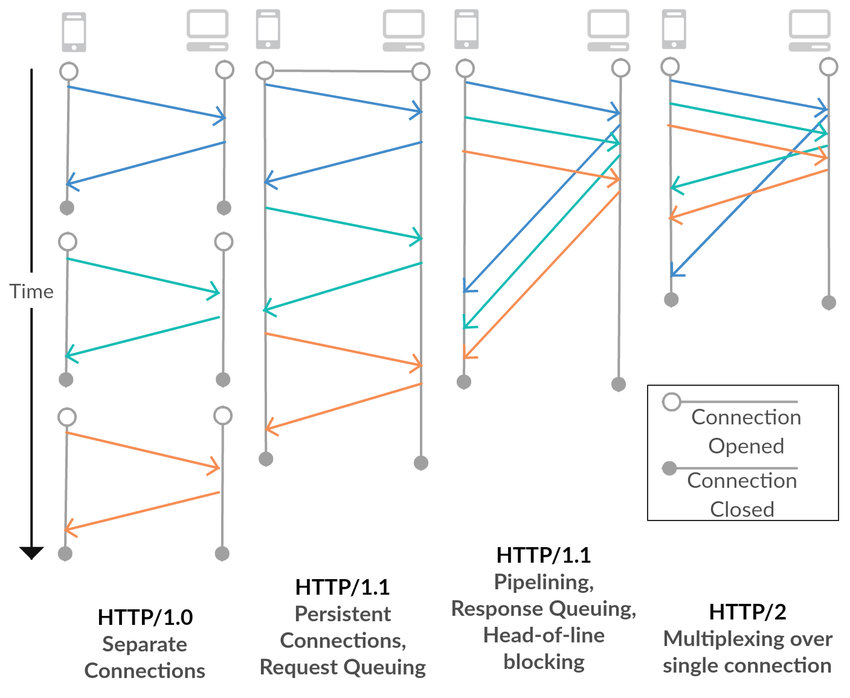
\includegraphics[width=\linewidth]{figures/Comparison-of-HTTP-versions.jpg}
    \caption{Comparison of HTTP Versions}
    {Source: \cite{comparison_of_http_versions}}
    \label{fig:comparison_of_http_versions}
\end{figure}

As all request and response payloads had the same size during experiments, HTTP/2 multiplexing did not have an impact on throughput. Thus, HTTP/1 kept being the protocol with best performance due to its simplicity, while HTTP/2 needs to deal with compressing its requests headers.

\subsubsection*{Multi-AZ Higher Throughput}

As previously observed during Transport-Layer protocols, while latency affects sequential clients, it does not impact parallel clients as much. Parallel requests improved all application protocols' throughput since requests are performed simultaneously. Therefore, the bottleneck remains how fast requests leave the client and server's response time, and not latency.

\subsubsection*{Throughput Parallel Upper Limit}

The throughput upper limit seen during transport-layer protocols experiments remained during application-layer experiments for all protocols but HTTP/3. Sequential client experiments also had client and server completely free, resulting in immediate request processing by the client and a faster response by the server. However, parallel requests queuing delay problem remained, degrading throughput due to the time requests and responses needs to wait to be processed.

While the previous stated behaviour was true to 128KiB payloads and smaller, parallel requests with 512KiB payloads had a better throughput than sequential requests. Sending larger payloads concurrently benefits surpasses the queuing delay drawbacks. Thus, processing larger payloads results in increased throughput.

\subsubsection*{HTTP/3 Limits}

HTTP/3's throughput had an overall increase when performing parallel requests. It was not significant, however. The UDP receive buffer performance degradation still impacts HTTP/3 as it did with QUIC, preventing HTTP/3 to perform beyond 1Gb/s.

\clearpage

\begin{figure}[h!]
    \centering
    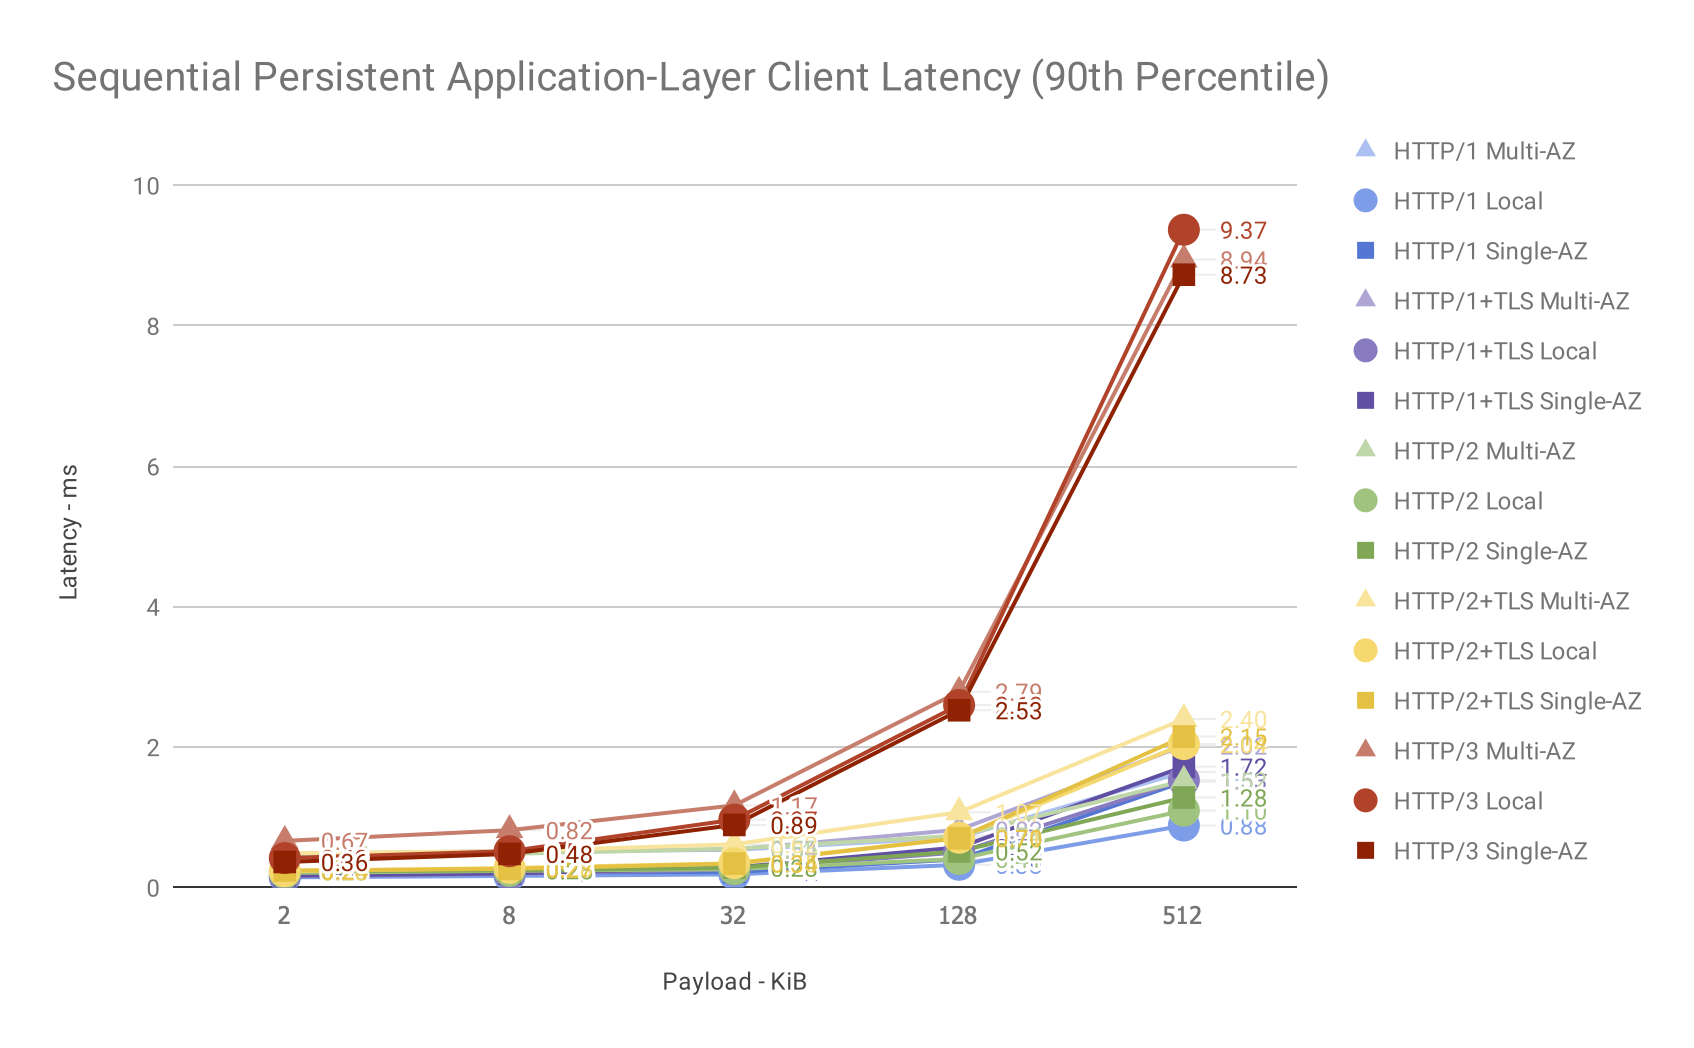
\includegraphics[width=\linewidth]{figures/charts/Sequential Persistent Application-Layer Client Latency (90th Percentile).png}
    \caption{Sequential Persistent Application-Layer Client Latency (90th Percentile)}
    \label{fig:sequential_app_latency}
\end{figure}
\begin{figure}[h!]
    \centering
    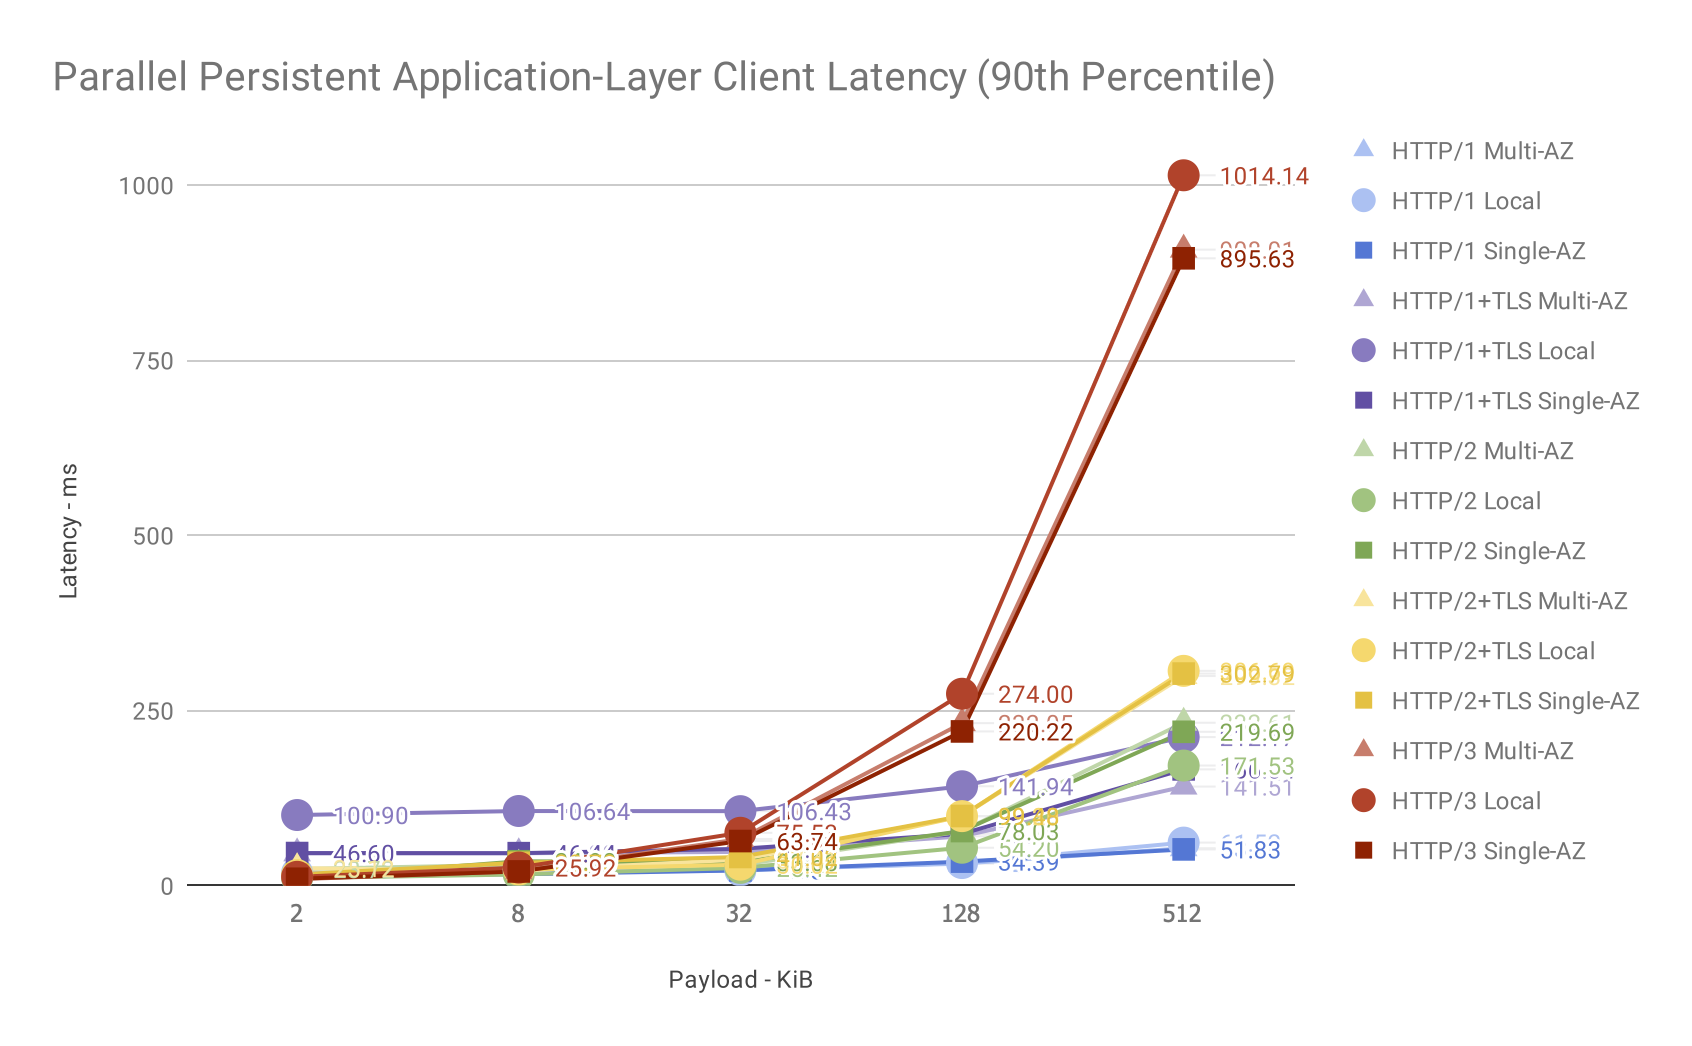
\includegraphics[width=\linewidth]{figures/charts/Parallel Persistent Application-Layer Client Latency (90th Percentile).png}
    \caption{Parallel Persistent Application-Layer Client Latency (90th Percentile)}
    \label{fig:parallel_app_latency}
\end{figure}


\begin{figure}[h!]
    \centering
    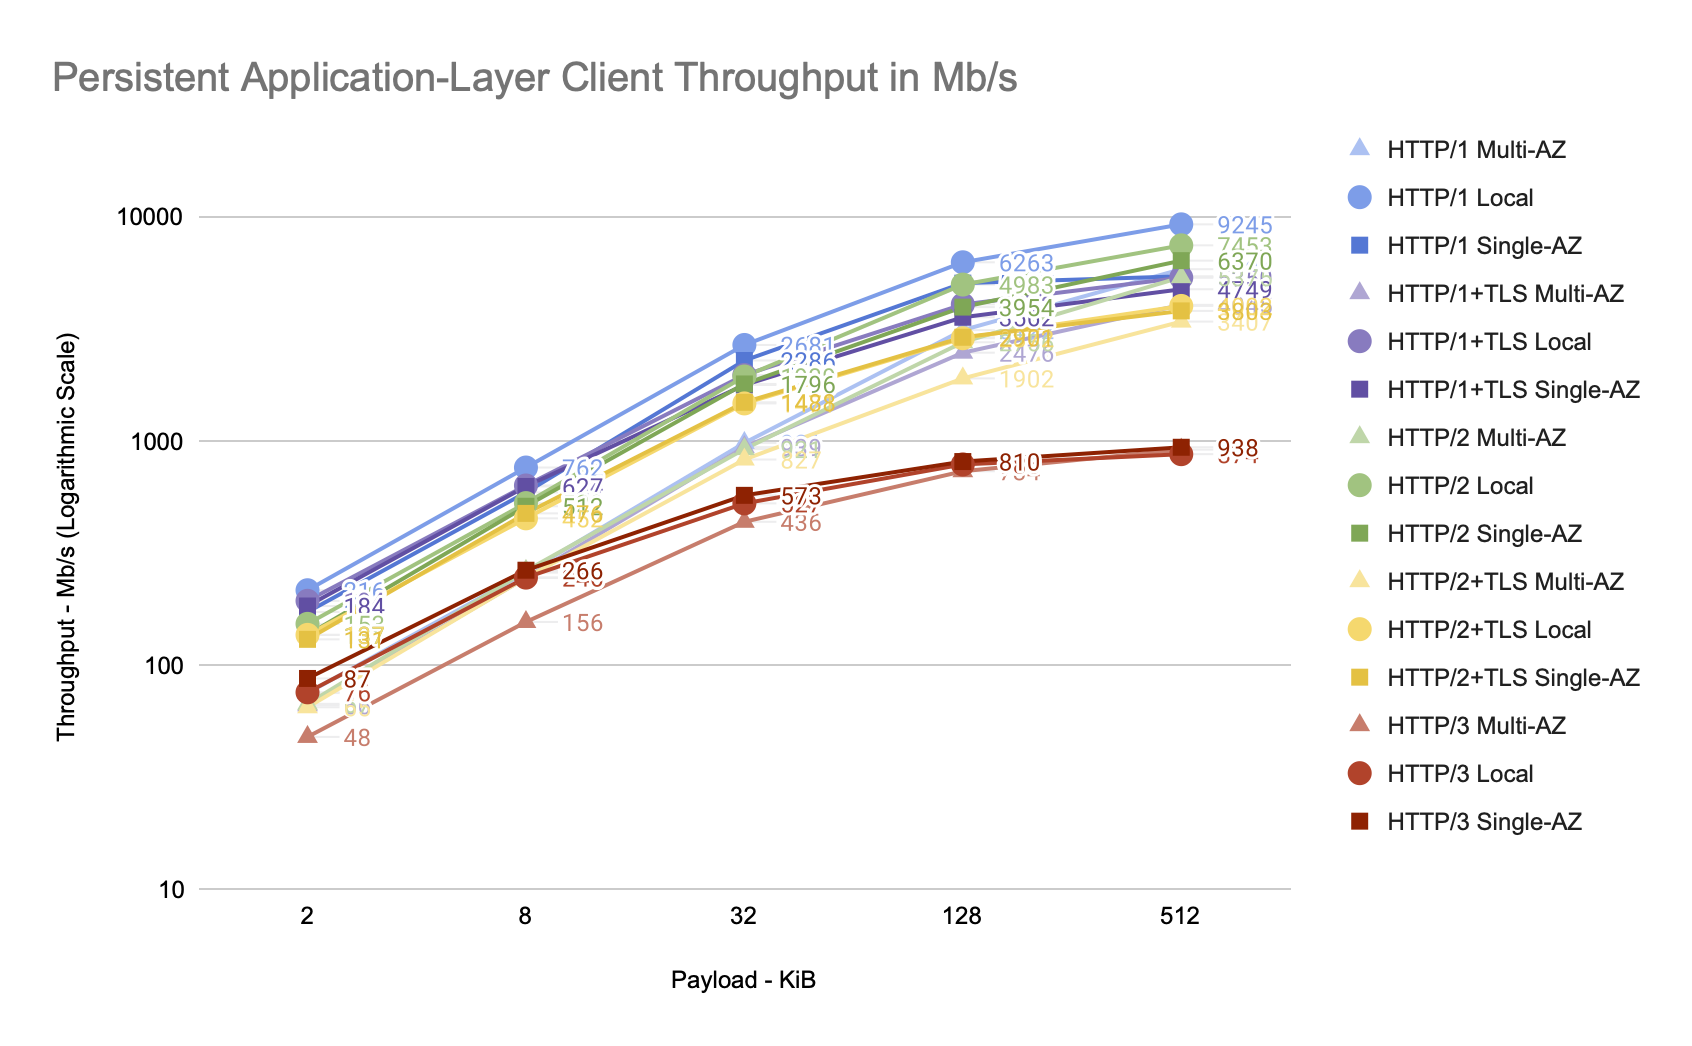
\includegraphics[width=\linewidth]{figures/charts/Persistent Application-Layer Client Throughput in Mb_s.png}
    \caption{Persistent Application-Layer Client Throughput in Mb/s}
    \label{fig:sequential_app_throughput}
\end{figure}
\begin{figure}[h!]
    \centering
    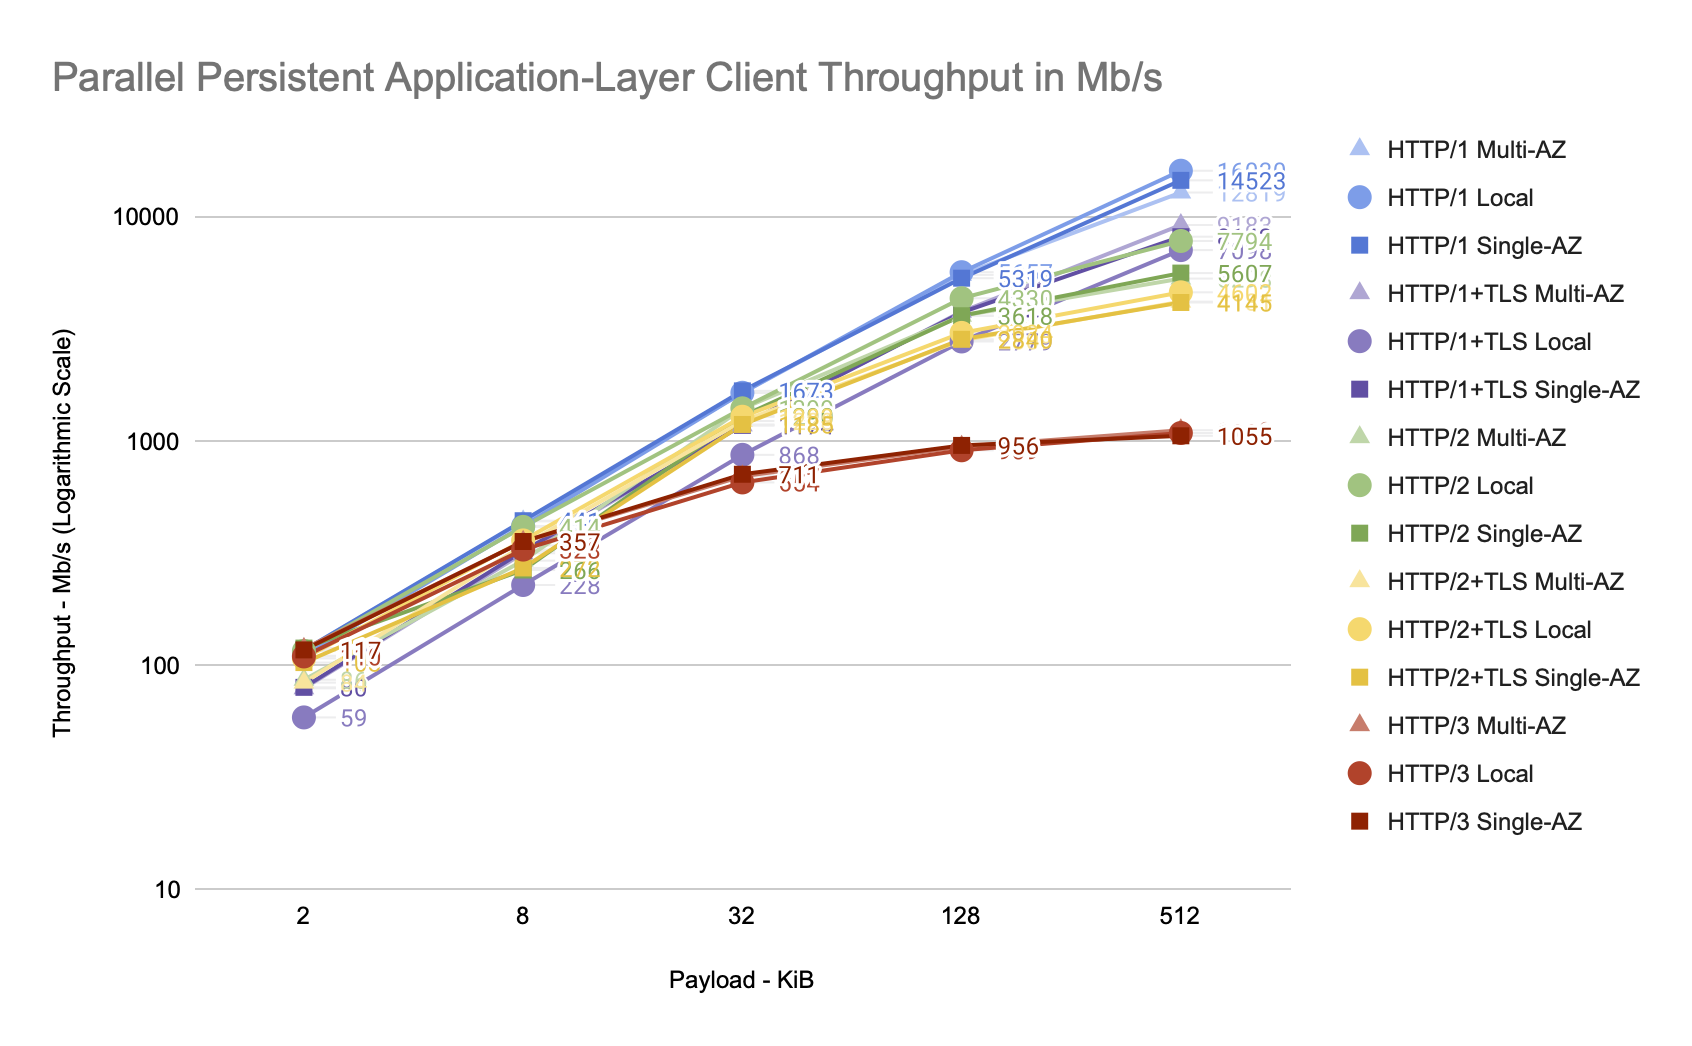
\includegraphics[width=\linewidth]{figures/charts/Parallel Persistent Application-Layer Client Throughput in Mb_s.png}
    \caption{Parallel Persistent Application-Layer Client Throughput in Mb/s}
    \label{fig:parallel_app_throughput}
\end{figure}

